\documentclass{bioinfo}
\usepackage{natbib}
\usepackage{url}
\copyrightyear{2009}
\pubyear{2009}

\newcommand{\Rpackage}[1]{`\texttt{#1}'}
\newcommand{\Rclass}[1]{\textsl{#1}}
\newcommand{\subfig}[1]{\textbf{#1}}

\begin{document}
\firstpage{1}

\title[Modular analysis]{Modular analysis of gene expression data with R}
\author[G\'abor Cs\'ardi \textit{et~al}]{G\'abor Cs\'ardi\,,$^{1,2}$,
  Zolt\'an Kutalik\,$^{1,2}$ and Sven Bergmann\,$^{1,2}$}
\address{$^{1}$Department of Medical Genetics, and
  $^{2}$Swiss Institute of Bioinformatics,
  University of Lausanne, Rue de Bugnon 27, CH-1005 Lausanne,
  Switzerland.}

\history{Received on XXXXX; revised on XXXXX; accepted on XXXXX}

\editor{Associate Editor: XXXXXXX}

\maketitle

\begin{abstract}
\section{Summary:}
Large sets of data, like expression profiles from many samples, require
analytic tools to reduce their complexity. Classical (bi-)clustering
algorithms typically attribute elements (genes, arrays) to disjoint groups
(``clusters''). Yet, in some cases overlapping cluster assignments would suit
the biological reality much better.

The Iterative Signature Algorithm (ISA) was designed to overcome this and
other limitations of standard clustering algorithms. It aims to reduce the
complexity of a very large set of data by decomposing it into so-called
``modules''. In the context of gene expression data these modules consist of
subsets of genes that exhibit a coherent expression profile only over a
subset of microarray experiments. Genes and arrays may be attributed to
multiple modules and the level of required coherence can be varied resulting
in different ``resolutions'' of the modular mapping. Since the ISA does not
rely on the computation of correlation matrices (like many other tools), it
is extremely fast even for very large datasets.

In this short note, we introduce two BioConductor \citep{BioC}, software
packages written in GNU~R: The~\Rpackage{isa2} includes a highly optimized
implementation of the ISA and~\Rpackage{eisa} provides a convenient interface
to run the ISA and visualize its output.

\section{Availability:}
The ISA homepage is at \href{http://www.unil.ch/cbg/homepage/software.html}%
{\url{http://www.unil.ch/cbg/homepage/software.html}}
\section{Contact:} \href{Sven.Bergmann@unil.ch}{Sven.Bergmann@unil.ch}
\end{abstract}

\section{Introduction}

% How the ISA works
The ISA can be applied to identify coherent substructures (i.e. modules)
from any rectangular matrix of data. To be specific we consider here the
case of transcriptomics data corresponding to a set of gene-expression
profiles from a collection of samples. The method has been described in
detail in Refs~\citep{isamod,isa}. Here we only give a brief summary.

The ISA identifies modules by an iterative procedure. The algorithm starts
from an input seed (corresponding to some set of genes or samples) which is
refined at each iteration by adding and/or removing genes and/or samples
until the process converges to a stable set, which is referred to as a
transcription module. This iterative procedure is typically performed to a
large number of seeds. In the unsupervised approach these seeds are chosen
randomly to sample uniformly the immense search space. We also implemented a
semi-supervised method, to which we refer as ``smart seeding'', where the
seeds a biased to start with certain sets of genes or samples for which
there is prior knowledge.

The output of ISA is a collection of potentially overlapping modules. Each
gene and each sample is attributed a score that reflects the strength of the
association with the module.

In the following we first outline how our software tool is commonly used for a
modular analysis (Section~\ref{sec:methods}) and then we describe in more
detail the R packages that implement the ISA and visualize its output
(Section~\ref{sec:implementation}).

\section{Methods}%
\label{sec:methods}

\begin{figure*}
\centering
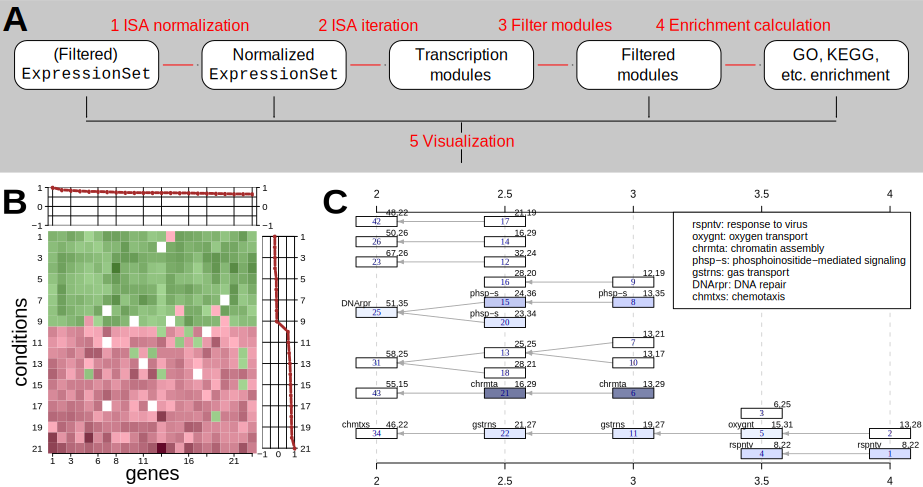
\includegraphics[width=\textwidth]{isa2workflow3}
\caption{\subfig{(A)} Work flow of a typical modular analysis study, with the
  \Rpackage{eisa} package. The input of the \Rpackage{eisa} pipeline is a
  BioConductor \Rclass{ExpressionSet} object. This is normalized to
  $Z$-scores (1); the ISA iterations are performed (2); and the
  biclusters are then merged and filtered based on the robustness
  measure (3). The \Rpackage{eisa} package contains tools to perform
  many GO, KEGG, etc. enrichment calculations quickly (4), and several
  bicluster visualization tools (5).
  Subfigures \subfig{B} and \subfig{C} were generated
  using the acute lymphoblastic leukemia data set, see
  \citep{chiaretti04} and the \Rpackage{ALL} R package.
  \subfig{(B)} Heatmap for a single module, showing correlated
  expression for the genes and samples. The red lines are the gene and
  sample scores.
  \subfig{(C)} A module tree. Each rectangle is a bicluster; see the
  definition of the edges in the text. The modules are colored
  according to their Gene Ontology enrichment $p$-values, the codes of
  the enriched GO categories are shown in the top-left corner of the
  rectangles. The top-right corner shows the number of genes and
  conditions in the bicluster. The gene thresholds used for finding
  the modules is shown on the horizontal axes.
}
\label{fig:workflow}
\end{figure*}

A typical modular analysis for gene expression data includes the following
steps:

% Batch correction
\emph{Batch correction.}
To study the global organization of a transcription program including
many aspects of transcriptional regulation one often combines several
microarray experiments into a single dataset. In such a case it is important
to properly normalize such data and reduce the bias due to constituent
datasets. Several methods address this challenge,
see e.g.~\citep{johnson07} for an algorithm that has a GNU R
implementation. 
% (S: Do we have a standard flag to call their software?)

% Filtering
\emph{Gene filtering.}
Genes that have very low expression levels in all samples, carry little if
any information and may reflect ineffective array probes, etc. Since these
genes are likely to contribute only noise to the analysis, we suggest
removing them before running the ISA iteration.
% (S: Describe how this is done, and if it requires setting a threshold!) 

% Normalization.
\emph{ISA normalization.}
In each iteration of the ISA weighted sums of expression levels over either
genes or samples are computed. Since different genes
typically show different levels of base
expression and variance, it is important to standardize expression
levels to $Z$-scores. The ISA uses two sets of $Z$-scores, one
calculated for each gene across all samples, the other for each sample
across all genes.

% Random and smart seeding.
\emph{Random and smart seeding.}
As mentioned previously, ISA can be performed with random or smart
seeds, based on the application.

% The ISA iteration.
\emph{The ISA iteration.}
This step is the core of the ISA and finds biclusters from the
starting seeds.

% Merging the modules.
\emph{Merging the modules.}
It is possible that several seeds converge to the same, or very similar
biclusters. This step eliminates such duplicates.

% The robustness measure and filtering the modules.
\emph{Robustness of biclusters.}
To access the significance of a bicluster, we designed a robustness
measure, that can be used to filter out spurious modules. This is done
based on performing ISA on the scrambled input data.

% Module trees.
\emph{Module trees.}
The ISA works with two stringency threshold parameters, the gene
threshold and the sample threshold. ISA modules can be organized into
a directed graph, a module tree, in which there is an edge from module
$A$ to module $B$, if the ISA converges to module $B$ from module $A$,
with the same threshold parameters  that were used to find module
$B$. A module tree provides a hierarchical modular description of a
data set.

\section{Implementation}%
\label{sec:implementation}

The ISA and accompanying visualization tools are implemented in two R
packages. The \Rpackage{isa2} package contains the implementation of
the basic ISA itself; this package can be used to analyze any tabular
data. The \Rpackage{eisa} package builds on \Rpackage{isa2}. It adds
support to standard BioConductor data structures; and
contains gene expression specific visualization tools (see 
Fig.~\ref{fig:workflow} for examples).

Both the \Rpackage{isa2} and \Rpackage{eisa} packages support two
workflows. The \emph{simple workflow} involves a single R function
call and runs all ISA steps (1-3 in Fig.~\ref{fig:workflow}.) with
their default parameters.

The \emph{detailed workflow} means running every step of the modular
analysis separately, possibly with non-default parameters. This allows
the users to tailor the ISA completely according their needs.

For users that prefer Matlab over R, we created a Matlab package for
ISA, please see the ISA homepage for more information.

% \subsubsection{Visualization}

The \Rpackage{eisa} package implements a set of visualization
techniques for biclusters, one of which is specific to ISA (see
Fig.~\ref{fig:workflow} for examples). 

% The \Rpackage{ExpressionView} R package, discussed in detail in
% another application note, implements an interactive tool
% for visualizing ISA (or other) overlapping biclusters.

% \subsubsection{Connection to other software}

The \Rpackage{biclust} package, \citep{biclust}, implements a number of
biclustering algorithms in a unified framework. The \Rpackage{eisa}
package include tools to convert between \Rpackage{biclust} and ISA
biclusters. This allows the cross-talk of the functions in the two
packages.

Additional information about the ISA, the \Rpackage{isa2} and
\Rpackage{eisa} packages and several tutorials are available on the
ISA homepage.

\section*{Acknowledgement}

\paragraph{Funding\textcolon} The authors are greatful to the Swiss
Institute of Bioinformatics, the Swiss National Science Foundation
(3100AO-116323/1), and the European Framework Project 6 (through
the EuroDia and AnEuploidy projects).
\paragraph{Conflict of interest\textcolon} None declared.

\bibliographystyle{natbib}
\bibliography{isa}

\end{document}
